\section{Algorithm}\label{sec:algo}

We now present \toolname, a SAT-based algorithm for mining \GRone
specifications from lasso traces.
The central observation is that the temporal structure of a \GRone
formula is \emph{fixed}: every component sits inside a known temporal
wrapper ($\always$, $\always\eventually$, or bare for initial
conditions).
Only the propositional content of each component---built from
$\land$, $\lor$, $\lnot$, and atomic propositions---needs to be
discovered.
We explain the algorithm constructively, using a running example.

\paragraph{Running example.}
Suppose $\mathit{AP}_e = \{x_0, x_1\}$ and
$\mathit{AP}_s = \{x_2, x_3\}$.
We are given two positive and two negative lasso traces and wish
to find the smallest \GRone formula separating them.

\subsection{Overview}\label{sec:overview}

Figure~\ref{fig:search} illustrates \toolname's search strategy.
The algorithm performs a two-dimensional search: the outer loop
increases the propositional formula depth $D$ (vertical axis),
controlling how complex each component can be
($D{=}1$: a single variable;
$D{=}2$: one operator, e.g.\ $\lnot x_0$;
$D{=}3$: trees, e.g.\ $x_0 \land x_1$);
the inner loop enumerates template configurations $(m,k,F)$
(horizontal axis), varying the number of justice and guarantee
conditions.
For each combination, \toolname encodes the mining problem as a SAT
instance and checks satisfiability, returning the first solution
found.

\begin{figure}[t]
\centering
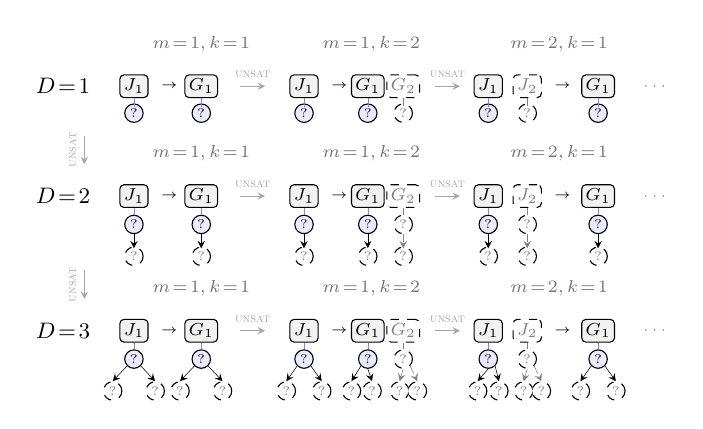
\begin{tikzpicture}[scale=0.9, every node/.style={transform shape},
  skel/.style={font=\scriptsize, draw, rounded corners=1.5pt,
               minimum height=0.32cm, inner sep=1.5pt, fill=gray!10},
  skeldash/.style={font=\scriptsize, draw, dashed, rounded corners=1.5pt,
               minimum height=0.32cm, inner sep=1.5pt, fill=white, text=gray},
  temporal/.style={font=\scriptsize},
  dagnode/.style={draw, circle, minimum size=0.26cm, inner sep=0pt,
                  font=\tiny, fill=blue!8},
  dagdash/.style={draw, circle, minimum size=0.26cm, inner sep=0pt,
                  font=\tiny, dashed, fill=white, text=gray},
   dagdot/.style={draw, circle, minimum size=0.26cm, inner sep=0pt,
                  font=\tiny, dotted, fill=white, text=gray},
  conn/.style={-, very thin, blue!50},
  arr/.style={->, >=stealth, very thin},
  darr/.style={->, >=stealth, very thin, dashed, gray},
  lbl/.style={draw=none, font=\small\bfseries},
  note/.style={draw=none, font=\tiny, text=black!55},
  uarr/.style={->, >=stealth, very thin, black!35},
]
% spacing constants
\def\colA{0.6}
\def\colB{3.0}
\def\colC{5.7}
\def\dotsX{7.5}
% vertical spacing
\def\rA{0}       % D=1 skeleton y
\def\rB{-1.55}   % D=2 skeleton y
\def\rC{-3.45}   % D=3 skeleton y
% D=2 chain spacing
\def\chH{0.45}   % chain node gap

% ========== D=1 ROW ==========
\node[lbl] at (-0.85, \rA) {$D\!=\!1$};

% --- m=1,k=1 ---
\node[note] at (\colA+0.5, \rA+0.6) {\scriptsize$m\!=\!1,k\!=\!1$};
\node[temporal] at (\colA-0.45, \rA+0.28) {\tiny$\always\eventually$};
\node[skel] (j1a) at (\colA-0.45, \rA) {$J_1$};
\node[temporal] at (\colA+0.05, \rA) {\tiny$\to$};
\node[temporal] at (\colA+0.5, \rA+0.28) {\tiny$\always\eventually$};
\node[skel] (g1a) at (\colA+0.5, \rA) {$G_1$};
\node[dagnode] at (\colA-0.45, \rA-0.38) {$?$};
\node[dagnode] at (\colA+0.5, \rA-0.38) {$?$};
\draw[conn] (j1a.south) -- ++(0,-0.13);
\draw[conn] (g1a.south) -- ++(0,-0.13);

\draw[uarr] (\colA+1.05, \rA) -- node[above, font=\tiny, text=black!35]
  {\textsc{unsat}} ++(0.35, 0);

% --- m=1,k=2 ---
\node[note] at (\colB+0.5, \rA+0.6) {\scriptsize$m\!=\!1,k\!=\!2$};
\node[temporal] at (\colB-0.45, \rA+0.28) {\tiny$\always\eventually$};
\node[skel] (j1b) at (\colB-0.45, \rA) {$J_1$};
\node[temporal] at (\colB+0.05, \rA) {\tiny$\to$};
\node[temporal] at (\colB+0.45, \rA+0.28) {\tiny$\always\eventually$};
\node[skel] (g1b) at (\colB+0.45, \rA) {$G_1$};
\node[temporal] at (\colB+0.95, \rA+0.28) {\tiny$\always\eventually$};
\node[skeldash] (g2b) at (\colB+0.95, \rA) {$G_2$};
\node[dagnode] at (\colB-0.45, \rA-0.38) {$?$};
\node[dagnode] at (\colB+0.45, \rA-0.38) {$?$};
\node[dagdash] at (\colB+0.95, \rA-0.38) {$?$};
\draw[conn] (j1b.south) -- ++(0,-0.13);
\draw[conn] (g1b.south) -- ++(0,-0.13);
\draw[conn, dashed, gray] (g2b.south) -- ++(0,-0.13);

\draw[uarr] (\colB+1.4, \rA) -- node[above, font=\tiny, text=black!35]
  {\textsc{unsat}} ++(0.35, 0);

% --- m=2,k=1 ---
\node[note] at (\colC+0.45, \rA+0.6) {\scriptsize$m\!=\!2,k\!=\!1$};
\node[temporal] at (\colC-0.55, \rA+0.28) {\tiny$\always\eventually$};
\node[skel] (j1c) at (\colC-0.55, \rA) {$J_1$};
\node[temporal] at (\colC+0.0, \rA+0.28) {\tiny$\always\eventually$};
\node[skeldash] (j2c) at (\colC+0.0, \rA) {$J_2$};
\node[temporal] at (\colC+0.5, \rA) {\tiny$\to$};
\node[temporal] at (\colC+1.0, \rA+0.28) {\tiny$\always\eventually$};
\node[skel] (g1c) at (\colC+1.0, \rA) {$G_1$};
\node[dagnode] at (\colC-0.55, \rA-0.38) {$?$};
\node[dagdash] at (\colC+0.0, \rA-0.38) {$?$};
\node[dagnode] at (\colC+1.0, \rA-0.38) {$?$};
\draw[conn] (j1c.south) -- ++(0,-0.13);
\draw[conn, dashed, gray] (j2c.south) -- ++(0,-0.13);
\draw[conn] (g1c.south) -- ++(0,-0.13);

\node[note] at (\dotsX, \rA) {$\cdots$};

% ========== down arrow ==========
\draw[arr, black!35] (-0.55, \rA-0.7) --
  node[left, font=\tiny, text=black!35] {\rotatebox{90}{\textsc{unsat}}}
  (-0.55, \rB+0.45);

% ========== D=2 ROW ==========
\node[lbl] at (-0.85, \rB) {$D\!=\!2$};

% --- m=1,k=1 ---
\node[note] at (\colA+0.5, \rB+0.6) {\scriptsize$m\!=\!1,k\!=\!1$};
\node[temporal] at (\colA-0.45, \rB+0.28) {\tiny$\always\eventually$};
\node[skel] (j1d) at (\colA-0.45, \rB) {$J_1$};
\node[temporal] at (\colA+0.05, \rB) {\tiny$\to$};
\node[temporal] at (\colA+0.5, \rB+0.28) {\tiny$\always\eventually$};
\node[skel] (g1d) at (\colA+0.5, \rB) {$G_1$};
\node[dagnode] (d2j1r) at (\colA-0.45, \rB-0.4) {$?$};
\node[dagdash] at (\colA-0.45, \rB-0.4-\chH) {$?$};
\draw[arr] (d2j1r.south) -- ++(0,-0.2);
\draw[conn] (j1d.south) -- (d2j1r.north);
\node[dagnode] (d2g1r) at (\colA+0.5, \rB-0.4) {$?$};
\node[dagdash] at (\colA+0.5, \rB-0.4-\chH) {$?$};
\draw[arr] (d2g1r.south) -- ++(0,-0.2);
\draw[conn] (g1d.south) -- (d2g1r.north);

\draw[uarr] (\colA+1.05, \rB) -- node[above, font=\tiny, text=black!35]
  {\textsc{unsat}} ++(0.35, 0);

% --- m=1,k=2 ---
\node[note] at (\colB+0.5, \rB+0.6) {\scriptsize$m\!=\!1,k\!=\!2$};
\node[temporal] at (\colB-0.45, \rB+0.28) {\tiny$\always\eventually$};
\node[skel] (j1e) at (\colB-0.45, \rB) {$J_1$};
\node[temporal] at (\colB+0.05, \rB) {\tiny$\to$};
\node[temporal] at (\colB+0.45, \rB+0.28) {\tiny$\always\eventually$};
\node[skel] (g1e) at (\colB+0.45, \rB) {$G_1$};
\node[temporal] at (\colB+0.95, \rB+0.28) {\tiny$\always\eventually$};
\node[skeldash] (g2e) at (\colB+0.95, \rB) {$G_2$};
\node[dagnode] (d2j1er) at (\colB-0.45, \rB-0.4) {$?$};
\node[dagdash] at (\colB-0.45, \rB-0.4-\chH) {$?$};
\draw[arr] (d2j1er.south) -- ++(0,-0.2);
\draw[conn] (j1e.south) -- (d2j1er.north);
\node[dagnode] (d2g1er) at (\colB+0.45, \rB-0.4) {$?$};
\node[dagdash] at (\colB+0.45, \rB-0.4-\chH) {$?$};
\draw[arr] (d2g1er.south) -- ++(0,-0.2);
\draw[conn] (g1e.south) -- (d2g1er.north);
\node[dagdash] (d2g2er) at (\colB+0.95, \rB-0.4) {$?$};
\node[dagdash] at (\colB+0.95, \rB-0.4-\chH) {$?$};
\draw[darr] (d2g2er.south) -- ++(0,-0.2);
\draw[conn, dashed, gray] (g2e.south) -- (d2g2er.north);

\draw[uarr] (\colB+1.4, \rB) -- node[above, font=\tiny, text=black!35]
  {\textsc{unsat}} ++(0.35, 0);

% --- m=2,k=1 ---
\node[note] at (\colC+0.45, \rB+0.6) {\scriptsize$m\!=\!2,k\!=\!1$};
\node[temporal] at (\colC-0.55, \rB+0.28) {\tiny$\always\eventually$};
\node[skel] (j1f2) at (\colC-0.55, \rB) {$J_1$};
\node[temporal] at (\colC+0.0, \rB+0.28) {\tiny$\always\eventually$};
\node[skeldash] (j2f2) at (\colC+0.0, \rB) {$J_2$};
\node[temporal] at (\colC+0.5, \rB) {\tiny$\to$};
\node[temporal] at (\colC+1.0, \rB+0.28) {\tiny$\always\eventually$};
\node[skel] (g1f2) at (\colC+1.0, \rB) {$G_1$};
\node[dagnode] (d2j1fr) at (\colC-0.55, \rB-0.4) {$?$};
\node[dagdash] at (\colC-0.55, \rB-0.4-\chH) {$?$};
\draw[arr] (d2j1fr.south) -- ++(0,-0.2);
\draw[conn] (j1f2.south) -- (d2j1fr.north);
\node[dagdash] (d2j2fr) at (\colC+0.0, \rB-0.4) {$?$};
\node[dagdash] at (\colC+0.0, \rB-0.4-\chH) {$?$};
\draw[darr] (d2j2fr.south) -- ++(0,-0.2);
\draw[conn, dashed, gray] (j2f2.south) -- (d2j2fr.north);
\node[dagnode] (d2g1fr) at (\colC+1.0, \rB-0.4) {$?$};
\node[dagdash] at (\colC+1.0, \rB-0.4-\chH) {$?$};
\draw[arr] (d2g1fr.south) -- ++(0,-0.2);
\draw[conn] (g1f2.south) -- (d2g1fr.north);

\node[note] at (\dotsX, \rB) {$\cdots$};

% ========== down arrow ==========
\draw[arr, black!35] (-0.55, \rB-0.4-\chH-0.2) --
  node[left, font=\tiny, text=black!35] {\rotatebox{90}{\textsc{unsat}}}
  (-0.55, \rC+0.45);

% ========== D=3 ROW ==========
\node[lbl] at (-0.85, \rC) {$D\!=\!3$};
\def\treeS{0.3}  % tree spread

% --- m=1,k=1 ---
\node[note] at (\colA+0.5, \rC+0.6) {\scriptsize$m\!=\!1,k\!=\!1$};
\node[temporal] at (\colA-0.45, \rC+0.28) {\tiny$\always\eventually$};
\node[skel] (j1f) at (\colA-0.45, \rC) {$J_1$};
\node[temporal] at (\colA+0.05, \rC) {\tiny$\to$};
\node[temporal] at (\colA+0.5, \rC+0.28) {\tiny$\always\eventually$};
\node[skel] (g1f) at (\colA+0.5, \rC) {$G_1$};
% J1 tree (solid/blue)
\node[dagnode] (t1jr) at (\colA-0.45, \rC-0.4) {$?$};
\node[dagdash] (t1jl) at (\colA-0.45-\treeS, \rC-0.85) {$?$};
\node[dagdash] (t1jrr) at (\colA-0.45+\treeS, \rC-0.85) {$?$};
\draw[arr] (t1jr.south west) -- (t1jl.north);
\draw[arr] (t1jr.south east) -- (t1jrr.north);
\draw[conn] (j1f.south) -- (t1jr.north);
% G1 tree (solid/blue)
\node[dagnode] (t1gr) at (\colA+0.5, \rC-0.4) {$?$};
\node[dagdash] (t1gl) at (\colA+0.5-\treeS, \rC-0.85) {$?$};
\node[dagdash] (t1grr) at (\colA+0.5+\treeS, \rC-0.85) {$?$};
\draw[arr] (t1gr.south west) -- (t1gl.north);
\draw[arr] (t1gr.south east) -- (t1grr.north);
\draw[conn] (g1f.south) -- (t1gr.north);

\draw[uarr] (\colA+1.05, \rC) -- node[above, font=\tiny, text=black!35]
  {\textsc{unsat}} ++(0.35, 0);

% --- m=1,k=2 ---
\node[note] at (\colB+0.5, \rC+0.6) {\scriptsize$m\!=\!1,k\!=\!2$};
\node[temporal] at (\colB-0.45, \rC+0.28) {\tiny$\always\eventually$};
\node[skel] (j1g) at (\colB-0.45, \rC) {$J_1$};
\node[temporal] at (\colB+0.05, \rC) {\tiny$\to$};
\node[temporal] at (\colB+0.45, \rC+0.28) {\tiny$\always\eventually$};
\node[skel] (g1g) at (\colB+0.45, \rC) {$G_1$};
\node[temporal] at (\colB+0.95, \rC+0.28) {\tiny$\always\eventually$};
\node[skeldash] (g2g) at (\colB+0.95, \rC) {$G_2$};
% J1: left+right (solid, like m=1,k=1)
\node[dagnode] (t2jr) at (\colB-0.45, \rC-0.4) {$?$};
\node[dagdash] (t2jl) at (\colB-0.7, \rC-0.85) {$?$};
\node[dagdash] (t2jrr) at (\colB-0.2, \rC-0.85) {$?$};
\draw[arr] (t2jr.south west) -- (t2jl.north);
\draw[arr] (t2jr.south east) -- (t2jrr.north);
\draw[conn] (j1g.south) -- (t2jr.north);
% G1: left+center (solid)
\node[dagnode] (t2g1r) at (\colB+0.45, \rC-0.4) {$?$};
\node[dagdash] (t2g1l) at (\colB+0.22, \rC-0.85) {$?$};
\node[dagdash] (t2g1c) at (\colB+0.51, \rC-0.85) {$?$};
\draw[arr] (t2g1r.south west) -- (t2g1l.north);
\draw[arr] (t2g1r.south) -- (t2g1c.north);
\draw[conn] (g1g.south) -- (t2g1r.north);
% G2: center+right (dashed)
\node[dagdash] (t2g2r) at (\colB+0.95, \rC-0.4) {$?$};
\node[dagdash] (t2g2c) at (\colB+0.9, \rC-0.85) {$?$};
\node[dagdash] (t2g2rr) at (\colB+1.15, \rC-0.85) {$?$};
\draw[darr] (t2g2r.south) -- (t2g2c.north);
\draw[darr] (t2g2r.south east) -- (t2g2rr.north);
\draw[conn, dashed, gray] (g2g.south) -- (t2g2r.north);

\draw[uarr] (\colB+1.4, \rC) -- node[above, font=\tiny, text=black!35]
  {\textsc{unsat}} ++(0.35, 0);

% --- m=2,k=1 ---
\node[note] at (\colC+0.45, \rC+0.6) {\scriptsize$m\!=\!2,k\!=\!1$};
\node[temporal] at (\colC-0.55, \rC+0.28) {\tiny$\always\eventually$};
\node[skel] (j1h) at (\colC-0.55, \rC) {$J_1$};
\node[temporal] at (\colC+0.0, \rC+0.28) {\tiny$\always\eventually$};
\node[skeldash] (j2h) at (\colC+0.0, \rC) {$J_2$};
\node[temporal] at (\colC+0.5, \rC) {\tiny$\to$};
\node[temporal] at (\colC+1.0, \rC+0.28) {\tiny$\always\eventually$};
\node[skel] (g1h) at (\colC+1.0, \rC) {$G_1$};
% J1: center+right children (solid)
\node[dagnode] (t3j1r) at (\colC-0.55, \rC-0.4) {$?$};
\node[dagdash] (t3j1c) at (\colC-0.7, \rC-0.85) {$?$};
\node[dagdash] (t3j1rr) at (\colC-0.4, \rC-0.85) {$?$};
\draw[arr] (t3j1r.south) -- (t3j1c.north);
\draw[arr] (t3j1r.south east) -- (t3j1rr.north);
\draw[conn] (j1h.south) -- (t3j1r.north);
% J2: center+right children (dashed)
\node[dagdash] (t3j2r) at (\colC+0.0, \rC-0.4) {$?$};
\node[dagdash] (t3j2c) at (\colC-0.05, \rC-0.85) {$?$};
\node[dagdash] (t3j2rr) at (\colC+0.2, \rC-0.85) {$?$};
\draw[darr] (t3j2r.south) -- (t3j2c.north);
\draw[darr] (t3j2r.south east) -- (t3j2rr.north);
\draw[conn, dashed, gray] (j2h.south) -- (t3j2r.north);
% G1: left+right children (solid)
\node[dagnode] (t3g1r) at (\colC+1.0, \rC-0.4) {$?$};
\node[dagdash] (t3g1l) at (\colC+0.75, \rC-0.85) {$?$};
\node[dagdash] (t3g1rr) at (\colC+1.25, \rC-0.85) {$?$};
\draw[arr] (t3g1r.south west) -- (t3g1l.north);
\draw[arr] (t3g1r.south east) -- (t3g1rr.north);
\draw[conn] (g1h.south) -- (t3g1r.north);

\node[note] at (\dotsX, \rC) {$\cdots$};

\end{tikzpicture}
\caption{Two-dimensional search in \toolname.
\textbf{Horizontal}: template enumeration over $(m,k)$ via
push/pop.
\textbf{Vertical}: propositional depth $D$.
$D\!=\!1$: single leaves.
$D\!=\!2$: chains (one operator).
$D\!=\!3$: trees ($\lnot x_0 \land x_1$, etc.).
Solid = current; dashed = newly added.}\label{fig:search}
\end{figure}



The \GRone template~\eqref{eq:gr1} is parameterised by the number
of justice conditions $m$, guarantees $k$, and a subset
$F \subseteq \{\mathit{init}, \mathit{safe}\}$ indicating which
optional component types to include: $\mathit{init} \in F$ means
the template includes initial-condition components
($\mathit{init}_\mathit{env}$ on the assumption side,
$\mathit{init}_\mathit{sys}$ on the guarantee side), and
$\mathit{safe} \in F$ means safety components are included.
Since the correct template is unknown, \toolname searches over
configurations $(m, k, F)
\in \{1,\ldots,M\} \times \{1,\ldots,K\} \times
2^{\{\mathit{init},\,\mathit{safe}\}}$
in non-decreasing order of total component count
$m + k + 2|F|$,
trying simpler templates first.

We pre-allocate a set of \emph{component identifiers}
$\mathcal{C} = \{J_1,\ldots,J_M,\; G_1,\ldots,G_K,\;
\mathit{init}_\mathit{env},\; \mathit{init}_\mathit{sys},\;
\mathit{safe}_\mathit{env},\; \mathit{safe}_\mathit{sys}\}$,
one for each slot in the maximal template.
Each $c \in \mathcal{C}$ names an \emph{unknown} propositional
formula to be determined by the SAT solver---for instance,
$\mathit{init}_\mathit{env}$ names the environment initial condition
whose content $\varphi_I^e$ is unknown.
The SAT variables $x^c, l^c, r^c$ encode the syntax DAG for~$c$
(Section~\ref{sec:component-dags}),
$y^c$ evaluates it on traces
(Section~\ref{sec:semantics}),
and $h^c$ captures whether it holds under its temporal wrapper
(Section~\ref{sec:temporal}).
The \textsc{EncodeAll} subroutine in
Algorithm~\ref{alg:main} bundles these steps for all
components at a given depth.

The key observation enabling incremental solving is that all
of these constraints are \emph{independent} of the template
configuration---only the consistency
constraints~(\eqref{eq:pos}--\eqref{eq:neg}) change.
For each depth $D$, we encode all $c \in \mathcal{C}$ once,
then iterate over template configurations.
Each configuration partitions the active components into
assumption-side ($J_i$, $\mathit{init}_\mathit{env}$, $\mathit{safe}_\mathit{env}$) and
guarantee-side ($G_j$, $\mathit{init}_\mathit{sys}$, $\mathit{safe}_\mathit{sys}$),
asserts the consistency constraints~\eqref{eq:pos}--\eqref{eq:neg}
inside a \textsc{Push}/\textsc{Pop} scope, and queries the solver.
\textsc{Push} saves a checkpoint on the solver's
constraint stack; \textsc{Pop} retracts all constraints added since
the checkpoint, restoring the solver to its prior state.
Learned clauses persist across checkpoints, so information
gained from one UNSAT configuration prunes subsequent
configurations at the same depth.

\paragraph{Example.}
At $D = 1$, the solver calls
\textsc{EncodeAll} for $\mathcal{C}$,
creating the SAT variables and constraints on all four traces.
It then tries template $(m{=}1, k{=}1, F{=}\emptyset)$:
\textsc{Push}, assert consistency for $\always\eventually J_1 \to
\always\eventually G_1$, call \textsc{Sat}.
If UNSAT, \textsc{Pop} and try $(1, 2, \emptyset)$:
$\always\eventually J_1 \to \always\eventually G_1 \land
\always\eventually G_2$.
If still UNSAT, continue through all configurations at $D = 1$,
then increment to $D = 2$, encode larger DAGs (allowing
$\lnot$, $\land$, $\lor$), and repeat.
Algorithm~\ref{alg:main} gives the complete procedure;
the remaining subsections detail the four families of constraints
added by \textsc{EncodeAll}: DAG structure
(Section~\ref{sec:component-dags}), propositional semantics
(Section~\ref{sec:semantics}), temporal holds
(Section~\ref{sec:temporal}), and trace consistency
(Section~\ref{sec:consistency}).

\begin{algorithm}[t]
\caption{\toolname}\label{alg:main}
\scriptsize
\DontPrintSemicolon
\SetKwInOut{Input}{Input}
\SetKwInOut{Output}{Output}
\SetKwFunction{Push}{Push}
\SetKwFunction{Pop}{Pop}
\SetKwFunction{Sat}{Sat}
\SetKwFunction{add}{add}
\SetKwFunction{Reconstruct}{Reconstruct}
\SetKwFunction{Encode}{EncodeAll}
\SetKwProg{Proc}{Procedure}{}{}
\Input{Traces $P$ (pos.), $N$ (neg.),
  partition $(\mathit{AP}_\mathit{env}, \mathit{AP}_\mathit{sys})$,
  bounds $M$, $K$}
\Output{Smallest \GRone formula separating $P$ from $N$}
\BlankLine
\Proc{\Encode{$\mathcal{S}, \mathcal{C}, D$}}{
  \ForEach{$c \in \mathcal{C}$}{
    Init $x^c_{i,\lambda}$, $l^c_{i,j}$, $r^c_{i,j}$
      $\forall\, i \!<\! D$,
      $\lambda \!\in\! \{\land,\lor,\lnot\} \!\cup\! \mathit{Vars}(c)$\;
    Init $y^c_{i,\sigma,t}$
      $\forall\, \sigma \!\in\! P \!\cup\! N$, $t \!<\! |\sigma|$\;
    Init $h^c_\sigma$
      $\forall\, \sigma \!\in\! P \!\cup\! N$\;
    $\mathcal{S}$.\add{one-hot labels, arity, acyclicity for
      $x^c, l^c, r^c$}
      \tcp*{Sec.~\ref{sec:component-dags}}
    $\mathcal{S}$.\add{propositional semantics of $y^c$ via
      $x^c, l^c, r^c$}
      \tcp*{Sec.~\ref{sec:semantics}}
    $\mathcal{S}$.\add{$h^c_\sigma$ via
      Eqs.~\eqref{eq:init}--\eqref{eq:guarantee}}
      \tcp*{Sec.~\ref{sec:temporal}}
  }
}
\noindent\textbf{end procedure}\;
\BlankLine
$\mathcal{S} \gets \textsc{SatSolver}.\textsc{new}()$\;
$\mathcal{C} \gets \{J_1,\ldots,J_M,\, G_1,\ldots,G_K,\,
  \mathit{init}_\mathit{env},\, \mathit{init}_\mathit{sys},\,
  \mathit{safe}_\mathit{env},\, \mathit{safe}_\mathit{sys}\}$\;
\For{$D = 1, 2, 3, \ldots$}{
  \Encode{$\mathcal{S}, \mathcal{C}, D$}
    \tcp*{permanent constraints}
  \For{$(m, k, F) \in
    \{1,\!\ldots\!,M\} {\times} \{1,\!\ldots\!,K\} {\times}
    2^{\{\mathit{init},\,\mathit{safe}\}}$}{
    $\mathcal{A} \gets \{J_1,\!\ldots\!,J_m\}$;\;
    $\mathcal{G} \gets \{G_1,\!\ldots\!,G_k\}$\;
    \lIf{$\mathit{init} \in F$}{$\mathcal{A} \gets \mathcal{A}
      \cup \{\mathit{init}_\mathit{env}\}$;\,
      $\mathcal{G} \gets \mathcal{G}
      \cup \{\mathit{init}_\mathit{sys}\}$}
    \lIf{$\mathit{safe} \in F$}{$\mathcal{A} \gets \mathcal{A}
      \cup \{\mathit{safe}_\mathit{env}\}$;\,
      $\mathcal{G} \gets \mathcal{G}
      \cup \{\mathit{safe}_\mathit{sys}\}$}
    $\mathcal{S}$.\Push{}
      \tcp*{ckpt: below is retractable}
    \ForEach{$\sigma \in P$}{
      $\mathcal{S}$.\add{$
        \bigwedge_{a \in \mathcal{A}} h^a_\sigma \Rightarrow
        \bigwedge_{g \in \mathcal{G}} h^g_\sigma$}\;
    }
    \ForEach{$\sigma \in N$}{
      $\mathcal{S}$.\add{$
        \bigwedge_{a \in \mathcal{A}} h^a_\sigma \land
        \lnot(\bigwedge_{g \in \mathcal{G}} h^g_\sigma)$}\;
    }
    \lIf{$\mathcal{S}$.\Sat{}}{
      \Return \Reconstruct{model, $\mathcal{A}, \mathcal{G}$}}
    $\mathcal{S}$.\Pop{}
      \tcp*{retract consistency constraints}
  }
}
\end{algorithm}


\subsection{Component DAGs}\label{sec:component-dags}

Each component $c$ of the \GRone template is an unknown
propositional formula.
We represent it as a syntax DAG of $D$ nodes
$0, 1, \ldots, D{-}1$, where node~$D{-}1$ is the root and
node~0 is always a leaf (atomic proposition).
The DAG is described by three families of SAT variables:
\begin{itemize}
\item $x^c_{i,\lambda}$: ``node $i$ is labelled $\lambda$,'' where
      $\lambda \in \{\land, \lor, \lnot\} \cup \mathit{Vars}(c)$
      and $\mathit{Vars}(c)$ is the set of variables permitted in
      component $c$ by the environment--system partition
      (Section~\ref{sec:gr1}).
\item $l^c_{i,j}$, $r^c_{i,j}$: ``the left (right) child of
      node $i$ is node $j$,'' for
      $1 \le i < D$, $0 \le j < i$.
\item $y^c_{i,\sigma,t}$: ``node $i$
      evaluates to true at position $t$ of trace~$\sigma$.''
\end{itemize}
Standard constraints enforce exactly one label per node,
correct arity ($\land$/$\lor$: two children; $\lnot$: one;
leaves: none), and acyclicity ($j < i$).

\paragraph{Example at $D = 1$.}
At depth $D = 1$, each component is a single leaf node---just an
atomic proposition.
For a justice component $J_1$, the partition restricts the leaf to
environment variables, so the SAT solver chooses among
$x^{J_1}_{0,x_0}$ and $x^{J_1}_{0,x_1}$ (exactly one must be true).
For a guarantee component $G_1$, only system variables are
permitted: $x^{G_1}_{0,x_2}$ or $x^{G_1}_{0,x_3}$.

\subsection{Propositional Semantics}\label{sec:semantics}

The $y$ variables link each DAG to the traces.
For a leaf labelled $x_p$:
$y^c_{i,\sigma,t} \Leftrightarrow \sigma[t][p]$.
For primed leaves $x_p'$ in safety components:
$y^c_{i,\sigma,t} \Leftrightarrow \sigma[\mathit{next}(t)][p]$.
For internal nodes, the semantics follow the operator:
\begin{align*}
x^c_{i,\land} \land l^c_{i,a} \land r^c_{i,b} &\;\Rightarrow\;
  \bigl(y^c_{i,\sigma,t} \Leftrightarrow
  y^c_{a,\sigma,t} \land y^c_{b,\sigma,t}\bigr) \\
x^c_{i,\lor} \land l^c_{i,a} \land r^c_{i,b} &\;\Rightarrow\;
  \bigl(y^c_{i,\sigma,t} \Leftrightarrow
  y^c_{a,\sigma,t} \lor y^c_{b,\sigma,t}\bigr) \\
x^c_{i,\lnot} \land l^c_{i,a} &\;\Rightarrow\;
  \bigl(y^c_{i,\sigma,t} \Leftrightarrow
  \lnot\, y^c_{a,\sigma,t}\bigr)
\end{align*}
These are asserted for every trace $\sigma$ and position $t$.

\paragraph{Example.}
Suppose the solver assigns $x^{J_1}_{0,x_0} = \mathit{true}$
(i.e., $J_1$ is the proposition $x_0$).
Then for each trace $\sigma$ and position $t$,
$y^{J_1}_{0,\sigma,t}$ is forced to equal $\sigma[t][0]$---the
value of $x_0$ at that position.
No search over temporal operators occurs; the $y$ variables are
purely propositional.

\subsection{Temporal Holds}\label{sec:temporal}

Rather than searching over temporal operators, we \emph{hardcode}
the temporal semantics of each component's wrapper.
A single Boolean variable $h^c_\sigma$ captures whether component
$c$ holds on trace~$\sigma$, defined in terms of the root node's
$y$ values.
For a trace $\sigma$ of length $L$ with lasso start $\ell$:
\begin{align}
  h^{\mathit{init}}_\sigma &\;\Leftrightarrow\;
    y^{\mathit{init}}_{D-1,\,\sigma,\,0}
    \label{eq:init}\\[2pt]
  h^{\mathit{safety}}_\sigma &\;\Leftrightarrow\;
    \textstyle\bigwedge_{t=0}^{L-1}
    y^{\mathit{safety}}_{D-1,\,\sigma,\,t}
    \label{eq:safety}\\[2pt]
  h^{J_i}_\sigma &\;\Leftrightarrow\;
    \textstyle\bigvee_{t \in \mathit{loop}(\sigma)}
    y^{J_i}_{D-1,\,\sigma,\,t}
    \label{eq:justice}\\[2pt]
  h^{G_j}_\sigma &\;\Leftrightarrow\;
    \textstyle\bigvee_{t \in \mathit{loop}(\sigma)}
    y^{G_j}_{D-1,\,\sigma,\,t}
    \label{eq:guarantee}
\end{align}

\paragraph{Example.}
Continuing with $J_1 = x_0$ and a trace $\sigma$ whose loop
positions are $\{2, 3\}$: $h^{J_1}_\sigma$ is true iff
$\sigma[2][0] \lor \sigma[3][0]$---i.e., $x_0$ is true at some
loop position.
This directly encodes $\always\eventually(x_0)$ without ever
introducing $\always$ or $\eventually$ as SAT-searchable
operators.

\subsection{Consistency Constraints}\label{sec:consistency}

The consistency constraints tie all components together by enforcing
the assume--guarantee semantics of \GRone on the given traces.
Let $\mathcal{A}$ and $\mathcal{G}$ be the sets of active assumption
and guarantee components for a template configuration.
For each positive trace $\sigma \in P$:
\begin{equation}\label{eq:pos}
  \textstyle\bigwedge_{a \in \mathcal{A}} h^a_\sigma
  \;\Rightarrow\;
  \textstyle\bigwedge_{g \in \mathcal{G}} h^g_\sigma
\end{equation}
For each negative trace $\sigma \in N$:
\begin{equation}\label{eq:neg}
  \textstyle\bigwedge_{a \in \mathcal{A}} h^a_\sigma
  \;\;\land\;\;
  \lnot\bigl(\textstyle\bigwedge_{g \in \mathcal{G}} h^g_\sigma\bigr)
\end{equation}

\paragraph{Example.}
For the template $\always\eventually J_1 \to \always\eventually G_1$
with $\mathcal{A} = \{J_1\}$ and $\mathcal{G} = \{G_1\}$:
each positive trace requires
$h^{J_1}_{\sigma^+} \Rightarrow h^{G_1}_{\sigma^+}$
(if the assumption holds, the guarantee must hold), and
each negative trace requires
$h^{J_1}_{\sigma^-} \land \lnot h^{G_1}_{\sigma^-}$
(the assumption holds \emph{and} the guarantee fails).
If the SAT solver finds a satisfying assignment, we read off
$x^{J_1}_{0,x_0} = \mathit{true}$ and
$x^{G_1}_{0,x_2} = \mathit{true}$, yielding the formula
$\always\eventually(x_0) \to \always\eventually(x_2)$.
